\documentclass[runningheads,orivec]{llncs}
\usepackage{xcolor}
\usepackage{graphicx}
%\usepackage{infrule}
\usepackage{latexsym}
% make sure mathsf uses the same font as lstlistings:
\DeclareMathAlphabet{\mathsf}{OT1}{phv}{m}{n}
\SetMathAlphabet{\mathsf}{bold}{OT1}{phv}{bx}{n}
\usepackage{listings}
\usepackage{lstlangcoq}
\renewcommand{\lstlistingname}{Figure}
\lstset{language=Coq,basicstyle=\sffamily,mathescape=true,columns=fullflexible}
\usepackage{semantic}

\newcommand{\PROP}{\mbox{\small PROP}}
\newcommand{\LOCAL}{\mbox{\small LOCAL}}
\newcommand{\SEP}{\mbox{\small SEP}}

\hyphenation{Comp-Cert}
\newcommand{\subtype}{<:}

\newif\iffullversion
\fullversionfalse

\begin{document}
%
\title{Modular Verification of C Programs \\ in Verifiable C}
\titlerunning{Modular Verification of C Programs}
\author{Lennart Beringer\and
Andrew W. Appel
}
\authorrunning{L. Beringer and A. W. Appel}
\institute{\today}
\maketitle              % typeset the header of the contribution
\begin{abstract}
  C programs are broken into modules (.c files)
  that import (call upon) functions from each other.
  VST verifications can follow the modular structure of the program.
  This tutorial shows how.
\end{abstract}

We assume the reader is familiar with the use of Verifiable C to prove
functional correctness of single-file C programs.  Here we illustrate
the modular verification of modular C programs.

Our main example is an abstract data
type (ADT) for \emph{piles}, simple collections of integers.
The complete example (C code and Coq verification)
can be found in the VST distribution
(or github repo), in directory progs/pile.

\begin{figure}[p]
\begin{minipage}[t]{2.5in}
\begin{lstlisting}[language=C]
/* pile.h */
typedef struct pile *Pile;
Pile Pile_new(void);
void Pile_add(Pile p, int n);
int Pile_count(Pile p);
void Pile_free(Pile p);

/* onepile.h */
void Onepile_init(void);
void Onepile_add(int n);
int Onepile_count(void);

/* apile.h */
void Apile_add(int n);
int Apile_count(void);

/* triang.h */
int Triang_nth(int n);

/* triang.c */
#include "pile.h"
int Triang_nth(int n) {
  int i,c;
  Pile p = Pile_new();
  for (i=0; i<n; i++)
    Pile_add(p,i+1);
  c = Pile_count(p);
  Pile_free(p);
  return c;
}

/* onepile.c */
#include "pile.h"
Pile the_pile;
void Onepile_init(void)
 {the_pile = Pile_new();}
void Onepile_add(int n)
 {Pile_add(the_pile, n);}
int Onepile_count(void)
 {return Pile_count(the_pile);}
\end{lstlisting}
\end{minipage}\begin{minipage}[t]{2.5in}
\begin{lstlisting}[language=C]
/* pile_private.h */
struct list {int n; struct list *next;};
struct pile {struct list *head;};

/* pile.c */
#include <stddef.h>
#include "stdlib.h"
#include "pile.h"
#include "pile_private.h"
Pile Pile_new(void) {
  Pile p = (Pile)surely_malloc(sizeof *p);
  p->head=NULL;
  return p;
}
void Pile_add(Pile p, int n) {
  struct list *head = (struct list *)
      surely_malloc(sizeof *head);
  head->n=n;
  head->next=p->head;
  p->head=head;
}
int Pile_count(Pile p) {
  struct list *q;
  int c=0;
  for(q=p->head; q; q=q->next)
    c += q->n;
  return c;
}
void Pile_free(Pile p) { . . . }


/* apile.c */
#include "pile.h"
#include "pile_private.h"
#include "apile.h"
struct pile a_pile = {NULL};
void Apile_add(int n) 
  {Pile_add(&a_pile, n);}
int Apile_count(void)
  {return Pile_count(&a_pile);}
\end{lstlisting}
\end{minipage}
\caption{The \lstinline{pile.h} abstract data type
has operations \emph{new, add, count, free}.  The \lstinline{triang.c}
client adds the integers 1--$n$ to the pile, then counts the pile.
The \lstinline{pile.c} implementation represents a pile
as header node (\lstinline{struct pile}) pointing to a linked
list of integers.  At bottom, there are two modules that each
implement a single ``implicit'' pile in a module-local global variable:
\lstinline{onepile.c} maintains a pointer to a pile,
while \lstinline{apile.c} maintains a \lstinline{struct pile} for which
it needs knowledge of the representation through \lstinline{pile_private.h}.
}
\label{example-program}
\end{figure}
Figure~\ref{example-program} (on the next page) shows a modular C
program that throws numbers onto a pile, then adds them up.\newline
\centerline{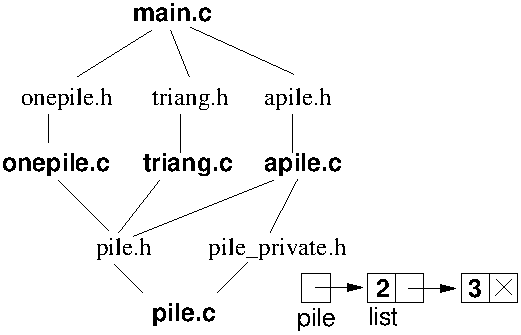
\includegraphics[scale=.7]{graphics/graph.pdf}\hspace{.5in}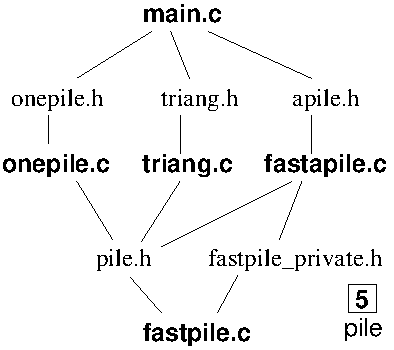
\includegraphics[scale=.7]{graphics/graph2.pdf}}
\noindent The diagram at left shows that \lstinline{pile.c} is
imported by \lstinline{onepile.c} (which manages a single pile),
\lstinline{apile.c} (which manages a single pile in a different way),
and \lstinline{triang.c} (which computes the $n$th triangular number).
The latter three modules are imported by \lstinline{main.c}.
\lstinline{Onepile.c} and \lstinline{triang.c} import the abstract
interface \lstinline{pile.h}; \lstinline{apile.c} imports also
the low-level concrete interface \lstinline{pile_private.h} that
exposes the representation---a typical use case for this organization
might be when \lstinline{apile.c} implements representation-dependent
debugging or performance monitoring.

When---as shown on the right---\lstinline{pile.c} is replaced by a
faster implementation \lstinline{fastpile.c} (code in
Figure~\ref{fig-fastpile}) using a different data structure,
\lstinline{apile.c} must be replaced with \lstinline{fastapile.c}, but
the other modules need not be altered, \emph{and neither should their
  specification or verification.}

% (* $
% \begin{array}{ll}
%   (&\mathrm{\_pile\_new}, \forall g:\mathrm{globals}. \\
%   & \{\mathrm{mem\_mgr}\,g\}\\
% & \{\exists p:\mathrm{val}.~
% \mathrm{ret}\Downarrow p\land
% \mathrm{pilerep}~\mathrm{nil}~p ~\ast~
% \mathrm{pile\_freeable}~p~\ast~\mathrm{mem\_mgr}\,g\} 
% )\end{array}$ *)

%$\qquad$ (* ${\small \mathsf{pilerep}}~\sigma~p ~~=~~ \exists x. ~ p\mapsto x ~\ast ~ p\uparrow ~ \ast ~ x \stackrel{\sigma}{\leadsto}\mathrm{nil}$ *)

\begin{figure}[tp]
\begin{minipage}[t]{3.2in}
\begin{lstlisting}[language=coq]
(* spec_pile.v *)
(* representation of linked lists in separation logic *)
Fixpoint listrep ($\sigma$: list Z) ($x$: val) : mpred :=
 match $\sigma$ with
 | $h$::$\mathit{hs}$ => EX $y$:val, !! (0 <= $h$ <=  Int.max_signed) && 
     data_at Ews tlist (Vint (Int.repr $h$), $y$) $x$ 
     * malloc_token Ews tlist $x$ *  listrep $\mathit{hs}$ $y$
 | nil => !! ($x$ = nullval) && emp
 end.

(* representation predicate for piles *)
Definition pilerep ($\sigma$: list Z) ($p$: val) : mpred :=
 EX $x$:val, data_at Ews tpile $x$ $p$ * listrep $\sigma$ $x$.

Definition pile_freeable ($p$: val) := 
  malloc_token Ews tpile $p$.

Definition Pile_new_spec :=
 DECLARE _Pile_new
 WITH $\mathit{gv}$: globals
 PRE [ ] PROP() LOCAL(gvars $\mathit{gv}$) SEP(mem_mgr $\mathit{gv}$)
 POST[ tptr tpile ]
   EX $p$: val, 
     PROP() LOCAL(temp ret_temp $p$)
     SEP(pilerep nil $p$; pile_freeable $p$; mem_mgr $\mathit{gv}$).

Definition Pile_add_spec :=
 DECLARE _Pile_add
 WITH $p$: val, $n$: Z, $\sigma$: list Z, $\mathit{gv}$: globals
 PRE [ _p OF tptr tpile, _n OF tint  ]
    PROP(0 <= $n$ <= Int.max_signed)
    LOCAL(temp _p $p$; temp _n (Vint (Int.repr $n$));
            gvars $\mathit{gv}$)
    SEP(pilerep $\sigma$ $p$; mem_mgr $\mathit{gv}$)
 POST[ tvoid ]
    PROP() LOCAL()
    SEP(pilerep ($n$::$\sigma$) $p$; mem_mgr $\mathit{gv}$).

Definition sumlist : list Z -> Z := List.fold_right Z.add 0.

Definition Pile_count_spec :=
 DECLARE _Pile_count
 WITH $p$: val, $\sigma$: list Z
 PRE [ _p OF tptr tpile  ]
    PROP(0 <= sumlist $\sigma$ <= Int.max_signed) LOCAL(temp _p $p$)
    SEP(pilerep $\sigma$ $p$)
 POST[ tint ]
    PROP() LOCAL(temp ret_temp (Vint (Int.repr (sumlist $\sigma$))))
    SEP(pilerep $\sigma$ $p$).
\end{lstlisting}
\end{minipage}\begin{minipage}[t]{1.7in}
\color{blue!50!black}
\begin{tabbing}
\textbf{Notation key}\\    
~~~~~~\=\\
\textsf{mpred}~~~~predicate on memory\\
\\
\textsf{EX}\>existential quantifier\\
\textsf{!!}\>injects Prop into mpred\\
\textsf{\&\&}\>nonseparating conjunction\\
\lstinline{data_at $\pi$ $\tau$ $v$ $p$} ~~is~~ $p\mapsto v$,\\
\>separation-logic mapsto \\
\>at type $\tau$, permission $\pi$\\
\\
\lstinline{malloc_token $\pi$ $\tau$ $x$} ~~~represents\\
\>``capability to deallocate $x$''\\
\\
\lstinline{Ews}~~~the ``extern write share'' \\
\>gives write permission\\
\\
\lstinline{_Pile_new} is a C identifier\\
\\
\lstinline{WITH}~~~quantifies variables\\
\>over \textsc{pre/post} of funspec\\
\\
The C function's return type,\\
\>\lstinline{tptr tpile},~~~is ``pointer\\
\>to \lstinline[language=C]{struct pile}''\\
\\
\lstinline{PROP($\ldots$)} are pure propositions\\
\>on the \lstinline{WITH}-variables\\
\\
\lstinline{LOCAL($\ldots$ temp _p $p\; \ldots$)}\\
\>associates C local var \lstinline{_p}\\
\>with Coq value $p$\\
\\
\lstinline{gvars $\mathit{gv}$}~~~~establishes $\mathit{gv}$ as\\
\>mapping from C global\\
\>vars to their addresses\\
\\
\lstinline{SEP($R_1$; $R_2$)} ~~ are separating\\
\>conjuncts $R_1 \ast R_2$\\
\\
\>\lstinline{mem_mgr $\mathit{gv}$} represents\\
\>~~~~~\=\emph{different} states of the\\
\>\>malloc/free system in\\
\>\>PRE and POST of\\
\>\>any function that\\
\>\>allocates or frees
\end{tabbing}
\end{minipage}
\vspace{-4ex}
\caption{\label{spec-pile} Specification of the pile module (\lstinline{Pile_free_spec} not shown).}

\end{figure}


Figure~\ref{spec-pile} presents the specification of the
pile module, in the Verifiable C separation logic.
Each C-language function identifier (such as \lstinline{_Pile_add})
is bound to a \lstinline{funspec}, a function specification
in separation logic.

Verifying that \lstinline{pile.c}'s functions satisfy the
specifications in Fig.~\ref{spec-pile} using VST-Floyd
is done by proving
Lemmas like this one (in file \lstinline{verif_pile.v}):

\begin{lstlisting}[language=coq]
Lemma body_Pile_new: semax_body Vprog Gprog f_Pile_new Pile_new_spec.
Proof. ... (*7 lines of Coq proof script*).... Qed.
\end{lstlisting}
\label{body-pile-new}
This says, in the context \lstinline{Vprog} of global-variable types,
in the context \lstinline{Gprog} of function-specs (for functions
that \lstinline{Pile_new} might call), the function-body
\lstinline{f_Pile_new} satisfies the function-specification
\lstinline{Pile_new_spec}.

\section{Specification files}
In the VST distribution directory progs/pile,
examine the files \lstinline{spec_*.v} and
\lstinline{verif_*.v}.  Let us take \lstinline{spec_onepile.v}
as an example:

\begin{lstlisting}
(* spec_onepile.v *)
Require Import VST.floyd.proofauto.
Require Import onepile.
Require Import spec_stdlib.
Require Import spec_pile.
Instance CompSpecs : compspecs. make_compspecs prog. Defined.
Definition Vprog : varspecs. mk_varspecs prog. Defined.
\end{lstlisting}
The \lstinline{CompSpecs} describes the fields
\lstinline{struct} and \lstinline{union} declarations
in the C program.  Each module may use different local
structs, or some structs may be declared in header files
so they appear in several modules.  Here, \lstinline{prog}
refers to \lstinline{onepile.prog}, so the CompSpecs
is built based on the structs in \lstinline{onepile.c}.
It's important that this \lstinline{Instance CompSpecs}
is built \emph{after} importing
\lstinline{spec_stdlib} and \lstinline{spec_pile},
otherwise their CompSpecs would shadow the one we want here.

\begin{lstlisting}
(* spec_onepile.v, continued *)
Definition onepile (gv: globals) (sigma: option (list Z)) : mpred :=
 match sigma with
 | None => data_at_ Ews (tptr tpile) (gv _the_pile)
 | Some il => EX p:val, data_at Ews (tptr tpile) p (gv _the_pile) *
                               pilerep il p * pile_freeable p
 end.
\end{lstlisting}
The separation-logic predicate for onepile
refers to the abstract predicates \lstinline{pilerep}
and \lstinline{pile_freeable} imported from \lstinline{spec_pile}.

Normally one would add here lemmas
\lstinline{onepile_local_facts} and
\lstinline{onepile_valid_pointer}, but we omit those here.

\begin{lstlisting}
(* spec_onepile.v, continued *)
Local Open Scope assert.

Definition Onepile_init_spec :=
 DECLARE _Onepile_init
 WITH gv: globals
 PRE [ ] 
    PROP() LOCAL(gvars gv) SEP(onepile gv None; mem_mgr gv)
 POST[ tvoid ]
    PROP() LOCAL() SEP(onepile gv (Some nil); mem_mgr gv).

Definition Onepile_add_spec :=
 DECLARE _Onepile_add
 WITH n: Z, sigma: list Z, gv: globals
 PRE [ _n OF tint  ]
    PROP(0 <= n <= Int.max_signed)
    LOCAL(temp _n (Vint (Int.repr n)); gvars gv)
    SEP(onepile gv (Some sigma); mem_mgr gv)
 POST[ tvoid ]
    PROP() LOCAL() SEP(onepile gv (Some (n::sigma)); mem_mgr gv).

Definition sumlist : list Z -> Z := List.fold_right Z.add 0.

Definition Onepile_count_spec :=
 DECLARE _Onepile_count
 WITH sigma: list Z, gv: globals
 PRE [  ]
    PROP(0 <= sumlist sigma <= Int.max_signed)
    LOCAL(gvars gv) SEP(onepile gv (Some sigma))
 POST[ tint ]
      PROP() LOCAL(temp ret_temp (Vint (Int.repr (sumlist sigma))))
      SEP(onepile gv (Some sigma)).
\end{lstlisting}
We have here a funspec corresponding to each function definition
in the .c file.


\begin{lstlisting}
(* spec_onepile.v, continued *)
Definition specs := [Onepile_init_spec; Onepile_add_spec; Onepile_count_spec].
Definition ispecs : funspecs := [].
\end{lstlisting}
This is the key point for modular verification:  In each
\lstinline{spec_X.v}, define two lists of funspecs:
\begin{description}
\item[specs:] Function specifications of exported functions
\item[ispecs:] Function specifications of internal functions, that
  are not called from other .c files.  (In principle, these could
  be declared \lstinline{static} in the .c program, but VST
  support for \lstinline{static} functions is not very good right now.)
\end{description}

\begin{lstlisting}
(* spec_onepile.v, continued *)
Lemma make_onepile: forall gv, 
  data_at_ Ews (tptr (Tstruct onepile._pile noattr)) (gv onepile._the_pile)
   |-- onepile gv None.
Proof. intros. unfold onepile. cancel. Qed.
\end{lstlisting}
The module \lstinline{onepile.c} has an extern global variable
\lstinline{the_pile}.  When the program is linked together,
this variable will appear in the \SEP part of the precondition
of \lstinline{main}, along with global variables from all other
modules.  It will appear in its concrete form, that is,
as a \lstinline{data_at}.  But the verification of
\lstinline{main} (and other client modules) would rather see it
in abstract form, that is, as \lstinline{onepile gv None}.
This lemma, provided by \lstinline{spec_onepile.v} and used
by \lstinline{verif_main.v}, converts the initialized global variable
from its concrete to abstract specification form.

\section{Verification files}
Now examine the verification of \lstinline{onepile.c}:

\begin{lstlisting}
(* verif_onepile.v *)
Require Import VST.floyd.proofauto.
Require Import linking.
Require Import onepile.
Require Import spec_stdlib spec_pile spec_onepile.
\end{lstlisting}
After importing \lstinline{VST.floyd.proofauto} as usual,
we import
\lstinline{linking}.  The file \linebreak \lstinline{VST/progs/pile/linking.v}
is an experimental linking system that will someday
be added as a standard feature to VST Floyd.
Then we import \lstinline{onepile}, that is,
the abstract syntax trees of \lstinline{onepile.c} that
we are verifying; and the \lstinline{spec_} modules of all
the C functions called upon by \lstinline{onepile.c}.

\begin{lstlisting}
(* verif_onepile.v, continued *)
Definition Gprog : funspecs := spec_pile.specs ++ spec_onepile.specs.
\end{lstlisting}
We build the \lstinline{Gprog} for verifying this module by
concatenating together the \lstinline{specs} lists of all
the modules we rely upon.

\begin{lstlisting}
(* verif_onepile.v, continued *)
Lemma body_Onepile_init: semax_body Vprog Gprog f_Onepile_init Onepile_init_spec.
Proof. ... Qed.

Lemma body_Onepile_add: semax_body Vprog Gprog f_Onepile_add Onepile_add_spec.
Proof. ... Qed.

Lemma body_Onepile_count: semax_body Vprog Gprog f_Onepile_count Onepile_count_spec.
Proof. ... Qed.

Definition module := 
  [mk_body body_Onepile_init; mk_body body_Onepile_add; 
   mk_body body_Onepile_count].
\end{lstlisting}
Verification of individual function bodies proceeds just as
usual in VST.  Then we collect this module's \lstinline{semax_body}
lemmas into a \lstinline{module}.

\section{Main}
The specification and verification of \lstinline{main} is
special, because we need to account for \emph{all} the modules'
global variables.

\begin{lstlisting}
(* spec_main.v *)
Require Import VST.floyd.proofauto.
Require Import main.
Require Import spec_stdlib spec_onepile spec_apile spec_triang.

Definition linked_prog : Clight.program :=
 ltac: (linking.link_progs_list [
   stdlib.prog; pile.prog; onepile.prog; apile.prog;
   triang.prog; main.prog]).
\end{lstlisting}  
We start by importing all the \lstinline{spec_} files,
then define the \lstinline{linked_prog} as
the combination of all the \lstinline{.c} programs.
This simulates what the Unix linker (\lstinline{ld})
will do.  In particular, the \lstinline{linked_prog}
has all the extern global variables of all the modules.

\begin{lstlisting}
(* spec_main.v *)
Instance CompSpecs : compspecs. make_compspecs linked_prog. Defined.
Definition Vprog : varspecs. mk_varspecs linked_prog. Defined.
Local Open Scope assert.

Definition main_spec :=
 DECLARE _main
 WITH gv: globals
 PRE [ ] main_pre linked_prog nil gv
 POST[ tint ]
    PROP() LOCAL(temp ret_temp (Vint (Int.repr 0))) SEP(TT).

Definition specs := [main_spec].
\end{lstlisting}  
Now, when we calculate the precondition of \lstinline{main},
that is, \lstinline{main_pre linked_prog nil gv},
all those global variables will be present in the
\SEP part of the precondition.

Finally, we export a \lstinline{specs} list as usual from this module,
containing just \lstinline{main_spec}.

\subsection*{Verification of main}
\begin{lstlisting}
(* verif_main.v *)
Require Import VST.floyd.proofauto.
Require Import linking.
Require Import main.
Require Import spec_stdlib spec_onepile spec_apile spec_triang spec_main.
Require verif_triang.

Definition Gprog : funspecs :=   
   spec_apile.specs ++ spec_onepile.specs ++ spec_triang.specs ++ spec_main.specs.
\end{lstlisting}
The beginning of \lstinline{verif_main} is just like
any other \lstinline{verif_} file:  Import the specs of
the modules with functions that you call.

Because \lstinline{main.c} does not call \lstinline{pile.c} directly,
there's no need to include \lstinline{spec_pile.specs} in the
\lstinline{Gprog}.

\begin{lstlisting}
(* verif_main.v, continued *)
Lemma body_main: semax_body Vprog Gprog f_main main_spec.
Proof.
start_function.
sep_apply (make_mem_mgr gv).
sep_apply (make_apile gv).
\end{lstlisting}
After the \lstinline{start_function} of \lstinline{body_main},
the precondition has (in its \SEP clause) many
\lstinline{data_at}s describing the initialized global variables.
Here we use (via \lstinline{sep_apply}) lemmas provided by
\lstinline{spec_stdlib} and \lstinline{spec_apile} to abstract
these predicates.

\begin{lstlisting}
(* verif_main.v, continued *)
generalize (make_onepile gv).
assert (change_composite_env spec_onepile.CompSpecs CompSpecs).
make_cs_preserve spec_onepile.CompSpecs CompSpecs.
change_compspecs CompSpecs.
intro Hx; sep_apply Hx; clear Hx.
\end{lstlisting}
In principle, we should do exactly the same with
the \lstinline{make_onepile} lemma, but it doesn't work;
there's a problem with the \lstinline{CompSpecs} that we fix
with this work-around.  This needs to be improved.

\begin{lstlisting}
(* verif_main.v, continued *)
forward_call gv.
. . .
Qed.

Definition module := [mk_body body_main].
\end{lstlisting}
Finally, after \lstinline{sep_apply}ing all the initialized-global-variable
abstraction lemmas, we verify the main function in the ordinary way.

\section{Linking}
A modular proof of a modular program is organized as follows:
CompCert parses each module \lstinline{M.c}
into the AST file \lstinline{M.v}.
Then we write the specification file \lstinline{spec_M.v}
containing funspecs as in Figure~\ref{spec-pile}.
We write \lstinline{verif_M.v} which imports
\lstinline{spec} files of all the modules from
which \lstinline{M.c} calls functions,
and contains \lstinline{semax_body} proofs of correctness,
for each of the functions in \lstinline{M.c}.

Now we prove that everything links together:

\begin{lstlisting}
(* link_pile.v *)
Require Import VST.floyd.proofauto.
Require Import linking.
Require main.
Require verif_stdlib verif_pile verif_onepile verif_apile.
Require verif_triang verif_main.

Definition allmodules := 
   verif_stdlib.module ++ verif_pile.module ++
   verif_onepile.module ++ verif_triang.module ++
   verif_apile.module ++ verif_main.module ++ nil.

Definition Gprog := ltac:
  (let x := constr:(merge_Gprogs_of allmodules) in
   let x := eval hnf in x in
   let x := eval simpl in x in 
   exact x).

Lemma prog_correct:
  semax_prog spec_main.linked_prog spec_main.Vprog Gprog.
Proof.
  prove_semax_prog.
  do_semax_body_proofs (SortBodyProof.sort allmodules).
Qed.
\end{lstlisting}



\begin{figure}[t]
\begin{lstlisting}[language=C]
/* fastpile_private.h */
struct pile { int sum; };

/* fastpile.c */
#include . . . 
#include "pile.h"
#include "fastpile_private.h"
Pile Pile_new(void)
  {Pile p = (Pile)surely_malloc(sizeof *p); p->sum=0; return p; }
void Pile_add(Pile p, int n)
  {int s = p->sum; if (0<=n && n<=INT_MAX-s) p->sum = s+n; }
int Pile_count(Pile p) {return p->sum;}
void Pile_free(Pile p) {free(p);}
\end{lstlisting}

% (* $\exists s. ~  0\le s \le M \wedge (\forall x\in \sigma.0\le x) \wedge (0 \le \Sigma\sigma \le M ~\rightarrow~s=\Sigma\sigma) \wedge~ p\mapsto x ~\ast ~ s\uparrow $ *)
\begin{lstlisting}[language=coq]
(* spec_fastpile.v *)
Definition pilerep ($\sigma$: list Z) ($p$: val) : mpred :=
 EX $s$:Z, !! (0 <= $s$ <= Int.max_signed /\ Forall (Z.le 0) $\sigma$ /\
             (0 <= sumlist $\sigma$ <= Int.max_signed -> $s$=sumlist $\sigma$))
   &&  data_at Ews tpile (Vint (Int.repr $s$)) $p$.

Definition pile_freeable := (* looks identical to the one in fig.$\mbox{\ref{spec-pile}}$ *)
Definition Pile_new_spec := (* looks identical to the one in fig.$\mbox{\ref{spec-pile}}$ *)
Definition Pile_add_spec := (* looks identical to the one in fig.$\mbox{\ref{spec-pile}}$ *)
Definition Pile_count_spec := (* looks identical to the one in fig.$\mbox{\ref{spec-pile}}$ *)
\end{lstlisting}
\caption{\label{fig-fastpile}\lstinline{fastpile.c}, a more efficient implementation
  of the pile ADT.  Since the only query function is \lstinline{count},
  there's no need to represent the entire list, just the sum will suffice.
  In the verification of a client program, the
  \lstinline{pilerep} separation-logic predicate has the same
  signature: \lstinline{list Z -> val -> mpred},
  even though the representation is a single number rather than
  a linked list.
}
\end{figure}

\section{Replacement of implementations}
\label{sec:subsumption}
We now turn to the replacement of \lstinline{pile.c} by a more
performant implementation, \lstinline{fastpile.c}, and its
specification---see Figure~\ref{fig-fastpile}. As
\lstinline{fastpile.c} employs a different data representation than
\lstinline{pile.c}, its specification employs a different
representation predicate \lstinline{pilerep}. As \lstinline{pilerep}'s
type remains unchanged, the function specifications look virtually
identical\footnote{\label{footnote-existential}Existentially abstracting over the internal
  representation predicates would further emphasize the uniformity
  between \lstinline{fastpile.c} and \lstinline{pile.c}---a detailed
  treatment of this is beyond the scope of the present article.};
however, the VST-Floyd proof scripts (in file
\lstinline{verif_fastpile.v}) necessarily differ. Clients importing only
the \lstinline{pile.h} interface, like \lstinline{onepile.c} or
\lstinline{triang.c}, cannot tell the difference (except that things
run faster and take less memory), and are specified and verified only
once (files \lstinline{spec_onepile.v} / \lstinline{verif_onepile.v}
and \lstinline{spec_triang.v} / \lstinline{verif_triang.v}).



\section{Subsumption of function specifications}

But we may also equip \lstinline{fastpile.c} with a more low-level
specification (see Figure~\ref{fastpile-concrete}) in which the
function specifications refer to a different representation predicate,
\lstinline{countrep}---clients of this interface do not need a notion
of ``sequence.'' 
The new specification is less abstract than the one
in Fig.~\ref{fig-fastpile},
and closer to the implementation.  The subsumption rule
allows us to exploit this relationship: we only
need to explicitly verify the code against the low-level specification
and can establish satisfaction of the high-level specification by
recourse to subsumption. This separation of concerns extends
from VST specifications to model-level reasoning: for example, in our
verification of cryptographic primitives we found it convenient to
verify that the C program implements a \emph{low-level functional
  model} and then separately prove that the low-level functional model
implements a high-level specification (e.g.~cryptographic security).
In our running example, \lstinline{fastpile.c}'s low-level functional
model is \emph{integer} (the Coq \lstinline{Z} type), and its high
level specification is \lstinline{list Z}.

To learn about \lstinline{funspec_sub}, its principles and how
to use it, see the paper, ``Abstraction and Subsumption in
Modular Verification of C Programs,''
by Lennart Beringer and Andrew W. Appel,
in \emph{FM'19: 3rd World Congress on Formal Methods},
October 2019.

\begin{figure}[t]
% Definition wrong_countrep ($s$: Z) ($p$: val) := data_at Ews tpile (Vint (Int.repr $s$)) $p$.
\begin{lstlisting}[language=coq]
(* spec_fastpile_concrete.v *)
Definition countrep ($s$: Z) ($p$: val) : mpred := EX $s'$:Z, 
  !! (0 <= $s$ /\ 0 <= $s'$ <= Int.max_signed /\ ($s$ <= Int.max_signed -> $s'$=$s$)) &&
  data_at Ews tpile (Vint (Int.repr $s'$)) $p$.

Definition count_freeable ($p$: val) := malloc_token Ews tpile p.

Definition Pile_new_spec := ...

Definition Pile_add_spec :=
 DECLARE _Pile_add
 WITH $p$: val, $n$: Z, $s$: Z, $\mathit{gv}$: globals
 PRE [ _p OF tptr tpile, _n OF tint  ]
    PROP(0 <= $n$ <= Int.max_signed)
    LOCAL(temp _p $p$; temp _n (Vint (Int.repr $n$)); gvars $\mathit{gv}$)
    SEP(countrep s $p$; mem_mgr $\mathit{gv}$)
 POST[ tvoid ]
    PROP() LOCAL() SEP(countrep ($n+s$) $p$; mem_mgr $\mathit{gv}$).

Definition Pile_count_spec := ...
\end{lstlisting}
\caption{\label{fastpile-concrete}The \lstinline{fastpile.c} implementation could be used
  in applications that simply need to keep a running total.
  That is, a \emph{concrete} specification can use
  a predicate \lstinline{countrep: Z -> val -> mpred}
  that makes no assumption about a sequence (\lstinline{list Z}).
  In \lstinline{countrep}, the variable $s'$ and the
    inequalities are needed to account for the possibility
    of integer overflow.
%  The \lstinline{wrong_countrep} is not an accurate specification
%  for this C module, because it does not account for
%  integer overflow.
}
\end{figure}



\end{document}
